\chapter{Experimental results}\label{ch:experiment}

In this chapter we present the results of experiments conducted in lab
environment against two major systems, Facebook Chat and Gmail. We will analyze
the validity of the attack under different modes, serial and parallel, as well
as the time consumption of each method. Also we will investigate the
effectiveness of the point-system meta-predictor introduced in Section
\ref{subsec:point_system}.

\section{Facebook Chat messages}\label{sec:fb_experiment}

The first experiment targeted Facebook Chat trying to exploit the vulnerability
presented in Section \ref{subsec:fb}. The first attempt used a regular Facebook
account with hundreds of friends and regular chat conversations and
notifications. However, using the validation method of Section
\ref{sec:mitmproxy}, it was found that between the secret and the reflection
lied a large amount of data which led to a non-compression of the two.

For the purpose of this paper we have created a lab account that has no friends
and no user activity of any kind, except for a self-sent private message that
will be the secret to be stolen. That way the noise of a real-world account,
such as new messages or notifications, is contained and we can avoid the
problems described above.

We assume an attack on Facebook chat messages following the serial method of
requests knowing the secret consists of letters, either lowercase or uppercase.
In order to steal the first letter of the secret we perform 4000 iterations of
requests, which translates to 4000 for each letter in the alphabet or
\begin{math}4000*52=208000\end{math} requests in total. The normal time
interval between two requests was set to 4 seconds in order to be sure that
overlapping stream can be distinguished. This has led to an overall
\begin{math}208000*4 = 832000\end{math} seconds which roughly equals to 9 days.

The following figure shows the behaviour of the correct letter as the attack
evolved:

\begin{figure}[H] \caption{Correct letter length chart.}
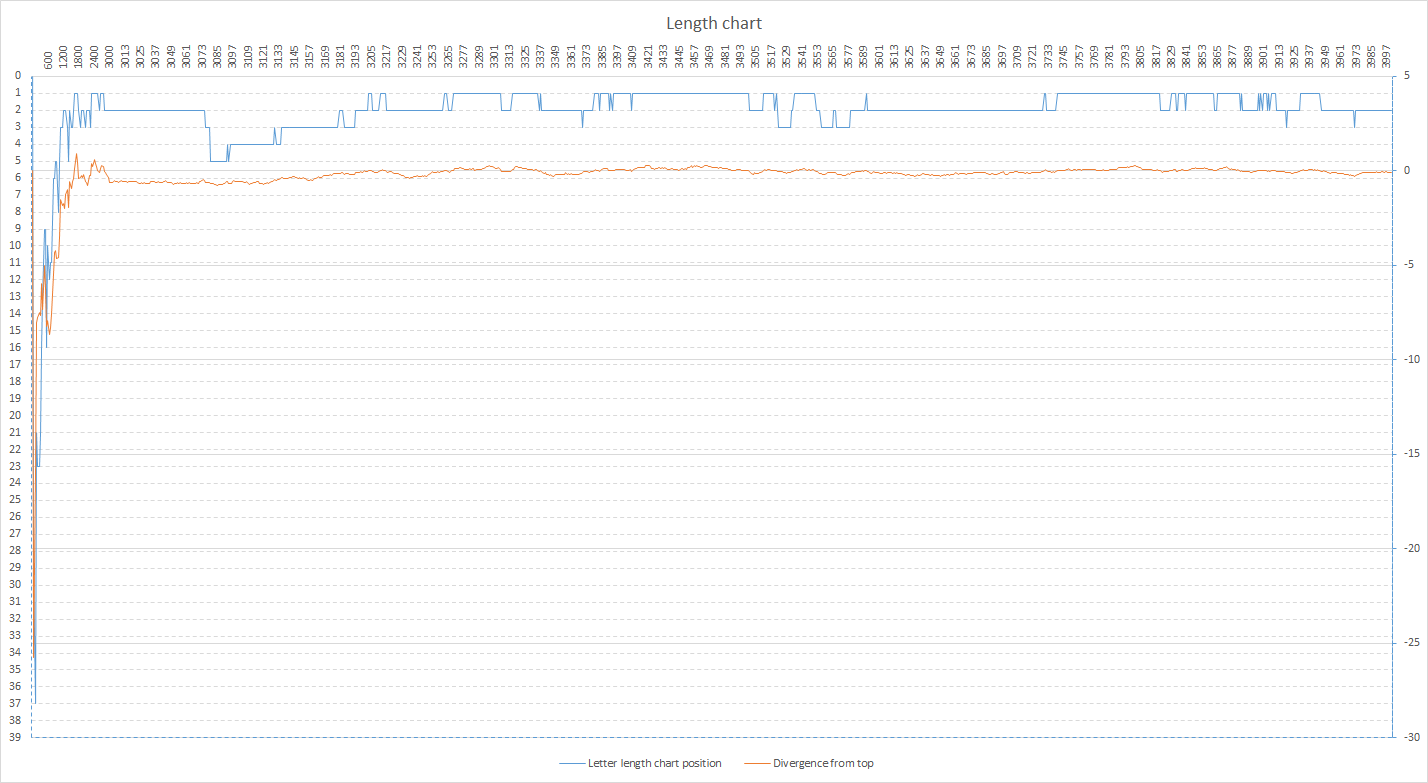
\includegraphics[width=1\textwidth]{diagrams/point_system_chart_1.png}\end{figure}

The top horizontal axis contains the number of iterations of requests.

The left vertical axis shows the position of the correct letter compared to the
others in ascending mean length order, i.e. the letter with minimum mean length
is \texttt{1}, the second smaller is \texttt{2} etc.

The right vertical axis depicts the difference of the mean lengths of the
correct letter and the \textit{best} one, i.e. the one with minimum mean length,
or the second \textit{best} in case the correct letter is the one of minimum
mean length.

It can be understood that the correct guess presents a good behaviour after a
transient period, although it does not always correspond to the minimum mean
response length. In order to handle this problem we introduced the point-system meta-predictor
presented in Section \ref{subsec:point_system}. In a similar manner we parsed
the collected data using the point-system information.

The chart depicting the evolution of the correct letter's
behaviour in time regarding the aggregated points is shown in the following
figure:

\begin{figure}[H] \caption{Correct letter point chart.}
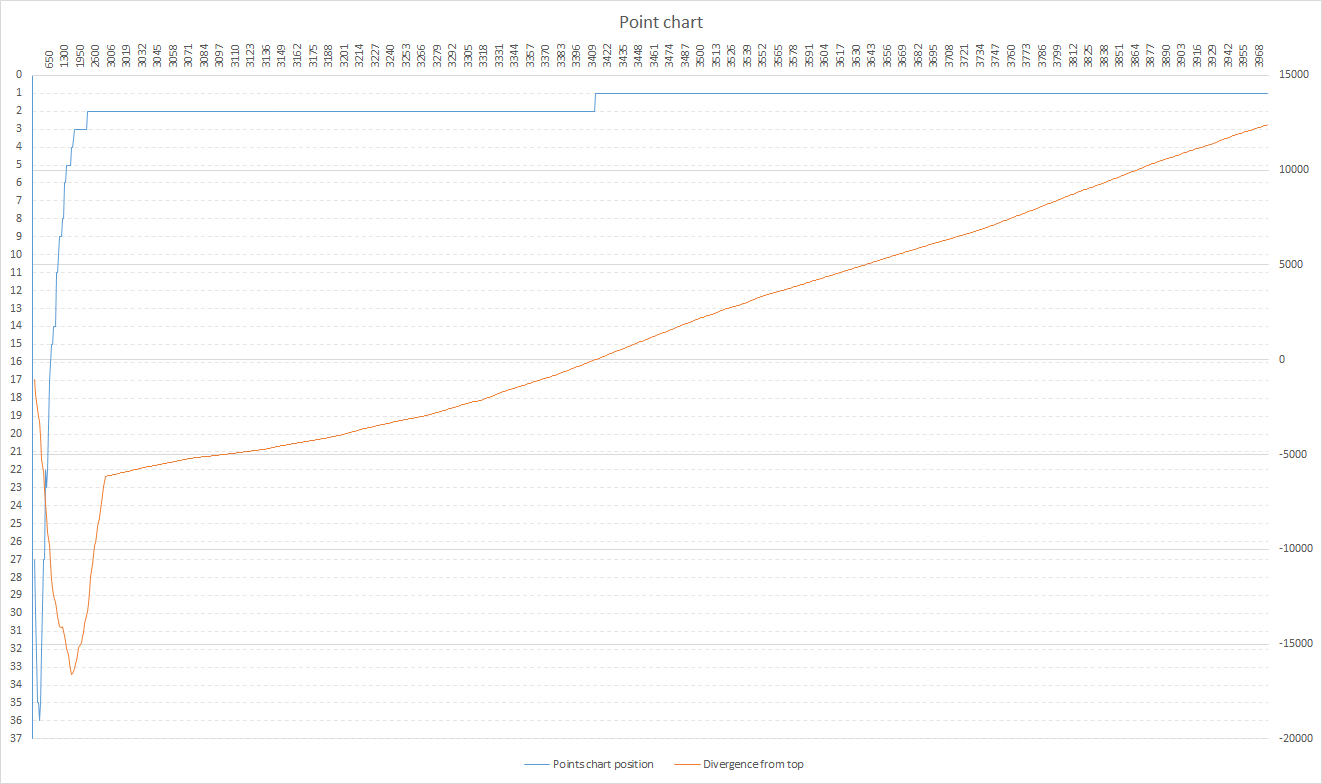
\includegraphics[width=1\textwidth]{diagrams/point_system_chart_2.png}\end{figure}

It is clear that by introducing the point system the prediction of the correct
letter is much more efficient than before. After a transient period the correct
letter demonstrates a better behaviour compared to any other choice, increasing
its point performance in an almost linear rate over time.

The demonstrated attack provides a statistical proof that Facebook Chat is not
IND-PCPA. It is clear that an adversary could gain a major advantage in stealing a
private Facebook Chat message using this attack model. However, it can be
understood that the attack performance of the attack is fairly poor, making it
particularly hard to be applied in real-world where the conditions for success
would need to be valid for a noticeable period of time.

\section{Gmail Authentication token}\label{sec:gmail_experiment}

Our next experiment aimed at stealing the authentication token of a Gmail
account as described in Section \ref{subsec:gmail_token}. Since noise during
this attack is at minimum level a regular account was used.

In this case, we employ the hill-climbing parallelization technique against a
full alphabet consisting of digits, lowercase and uppercase letters and dashes
totaling 64 items. In each stage of the attack the alphabet is divided in two
sets, so the one that presents the best behaviour is chosen to continue the
attack in the next stage resulting in a total of \begin{math}log(64) =
6\end{math} stages.

In order to validate the results of the measurements we repeat each stage of the
attack as many times as needed until one of the two sets shows minimum mean
length for an aggregate of 4 attempts so a maximum of 7 attempts should be made
for each stage. That way we can reduce the margin of error resulting in random
circumstances that may appear during an attempt.

Evaluation of the response stream was again based on the point-system. In this
case, since there are only two choices in each iteration, the points depict the
amount of iterations that each choice showed minimum mean length. Each attempt
on each stage ended when either half of the alphabet gathered
\begin{math}2000\end{math} points, therefore a total of
\begin{math}4000\end{math} requests was issued in each case, with a time
interval of 4 seconds between consecutive requests. Therefore, the
total amount of time theoretically needed for the completion of the attack to
steal one character of the token is \begin{math}4000*4*7*6 = 672000\end{math}
seconds, which is roughly 7 days.

The result of this experiment could be summarized in the following chart:

\begin{figure}[H] \caption{Successful attempts for each alphabet during parallelization.}
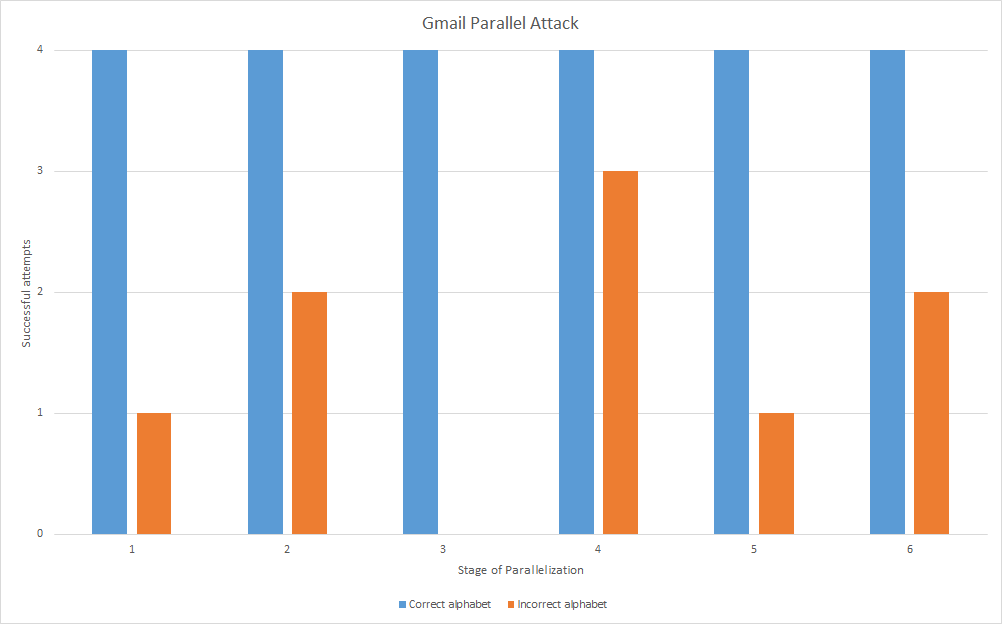
\includegraphics[width=1\textwidth]{diagrams/gmail_parallel.png}\end{figure}

Each stage of the parallel attack resulted in a correct choice of alphabet
ultimately leading to a successful guess on the first character of the token.
However, the correct alphabet was not successful in each attempt for all stages
of the attack but only some. In other stages the incorrect alphabet performed
better in up to 3 attempts presenting a very small advantage for the correct
alphabet. However, even in that worst case scenario, the correct alphabet
presented almost 60\% chance to be chosen.

In light of these findings, we can safely assume that Gmail is also not
IND-PCPA. An adversary that uses the proposed attack mechanism has a notable
advantage in correctly guessing each character of the authentication token.

Hill-climbing parallelization resulted in a notable reduction of requests
needed compared to the serial method and consequently a reduction of the
total time of execution. Also since Gmail authentication tokens are renewed
every time the user logs in the account the secret is less likely to be
modified compared to Facebook Chat messages.

However, even after these advantages the attack could not be described as a
real-world threat, since for a 20-character token \begin{math}7*20 =
140\end{math} days are needed, which is a very long period of time for the
attack assumptions to be met.
